%! TEX program = pdflatex
\documentclass[journal]{IEEEtran}
\usepackage{siunitx}
\usepackage{amsmath}
\usepackage{amssymb}
\usepackage{bm}
\usepackage[table,xcdraw]{xcolor}
\usepackage[pdftex]{graphicx}

\DeclareGraphicsRule{.ai}{pdf}{.ai}{}

\begin{document}

\title{QUIKS: an inexpensive motion tracking system}
\author{}
\maketitle
\begin{abstract}
Reducing cost for motion tracking system is essential for better virtual reality (VR) experience.
In this paper, we describe our low-cost system named QUIKS.
It is optimized for VR usage only.
Therefore, it can be constructed of inexpensive parts such as IMU and Cortex-M0+ MCU.
In addition, sensors not only sample motions but also calculate offset and apply transformation.
This lowers CPU usage of host PC.
We only spent about 10 dollars for tracking one joint.
In out tests, laptop PC without GPU can perform motion traccking and 3DCG rendering for 30 fps.
The quality and latency of motion is sufficient for VR experience.
\end{abstract}

\section{Introduction}
To capture the movement of a user is essential for the virtual reality (VR) experience.
With the increase of the number of VR user (including game player, streamer, etc.), perchasing motion tracking devices such as Vive tracker or Perception Neuron is thought to be a common case.
However, these products are still expensive and only a few user can perchase them.
Thus, a low-cost motion tracking system which is suitable for VR usage is needed.
Such a device should not track a motion much precisely or quickly.
That is, it is not suitable for the tasks like measurements and only produce 30 or 60 samples per second.
Also, it cannot be used with some particular motions which are difficult to track.

\section{Basis of motion tracking}
\subsection{Target software}
A motion data measured by a sensor is sent to some software to produce CG images for a user.
In this paper, we target Unity for that role because we can use it for free with few limitations.
However, most of our system can be reused for other software.

\subsection{Tracking method}
There are roughly two methods to track motions.
One is an optical method.
It can track almost every motions very precisely with low latency.
However, it needs multiple cameras and lots of calculation resources.
Thus, this method is not suitable for an inexpensive system.

The another is an inertial method.
It cannot track the absolute position of a body, but it is simple and costs less.
Therefore, we adopt this method.

The inertial method captures joint rotations and just assign them to a 3D model.
3DCG engine like Unity manages its internal model movements by rotations.
In general, inertial motion tracking can be achieved with following steps.
\begin{enumerate}
    \item Measure joint rotations by inertial measurement unit(IMU).
    \item Convert measured data for a 3DCG software.
    \item Assign joint rotations to a 3D model.
\end{enumerate}

\subsection{Quaternion}
A rotation in 3D space can be represented as the form of quaternion.
In this paper, we define a quaternion \(\bm{q}\) as (\ref{quat-def}).
\begin{equation}
    \bm{q} \overset{\mathrm{def}}{=} w + \mathbf{i}x + \mathbf{j}y + \mathbf{k}z = w + \begin{pmatrix}
        x \\
        y \\
        z
    \end{pmatrix} \label{quat-def}
\end{equation}
where \(w\) is the real part of a quaternion and \(x,\,y,\,z\) are the imaginary part.
\begin{table}[tb]
    \centering
    \caption{Quaternion multiplication} \label{quat-mult}
    \begin{tabular}{ccccc}
    \rowcolor[HTML]{9B9B9B} 
                                           & 1              & \(\mathbf{i}\)  & \(\mathbf{j}\)  & \(\mathbf{k}\)  \\
    \cellcolor[HTML]{9B9B9B}1              & \(1\)          & \(\mathbf{i}\)  & \(\mathbf{j}\)  & \(\mathbf{k}\)  \\
    \rowcolor[HTML]{EFEFEF} 
    \cellcolor[HTML]{9B9B9B}\(\mathbf{i}\) & \(\mathbf{i}\) & \(-1\)          & \(\mathbf{k}\)  & \(-\mathbf{j}\) \\
    \cellcolor[HTML]{9B9B9B}\(\mathbf{j}\) & \(\mathbf{j}\) & -\(\mathbf{k}\) & \(-1\)          & \(\mathbf{i}\)  \\
    \rowcolor[HTML]{EFEFEF} 
    \cellcolor[HTML]{9B9B9B}\(\mathbf{k}\) & \(\mathbf{k}\) & \(\mathbf{j}\)  & \(-\mathbf{i}\) & \(-1\)         
    \end{tabular}
\end{table}
Multiplication between each parts are defined as Table \ref{quat-mult}.
Also, (\ref{quat-norm}) always have to be valid.
When a quaternion holds this condition, it is called to be normalized.
\begin{equation}
    |\bm{q}| \overset{\mathrm{def}}{=} \sqrt{w^2 + x^2 + y^2 + z^2} = 1 \label{quat-norm} 
\end{equation}
Sometimes we need the inverse (or complementary) quaternion \(\bm{q}^{-1}\) defined as (\ref{quat-inv})
\begin{equation}
    \bm{q}^{-1} \overset{\mathrm{def}}{=} \frac{w - \mathbf{i}x - \mathbf{j}y - \mathbf{k}z}{w^2 + x^2 + y^2 + z^2} = w - \mathbf{i}x - \mathbf{j}y - \mathbf{k}z \label{quat-inv}
\end{equation}

The rotation around the axis \(\bm{u} = (u_x,\,u_y,\,u_z)^\mathrm{T}\in\mathbb{R}^3\) by angle \(\theta\) can be expressed in (\ref{quat-rot}).
\begin{equation}
    \bm{q} = \cos\left(\frac{\theta}{2}\right) + \begin{pmatrix}
        u_x \\
        u_y \\
        u_z
    \end{pmatrix} \sin\left(\frac{\theta}{2}\right) \label{quat-rot}
\end{equation}
where \(|\bm{u}| = 1\).

The rotaion \(\bm{q}_2\bm{q}_1\) means the rotation applying \(\bm{q}_1\), then \(\bm{q}_2\).

Real world coordinate and 3DCG engine coordinate are often different.
Real world is represented as left-handed coordinate system and Unity uses right-handed one for example.
In this case, we should convert rotation axis \(\bm{u}\) to \(\bm{u}'\) with \(\bm{u}' = A\bm{u}\) where \(A\in\mathbb{R}^{3\times 3}\) is an transformation matrix.
Therefore, a quaternion \(\bm{q}\) can be converted to \(\bm{q}'\) by (\ref{quat-conv}).
\begin{equation}
    \bm{q}' = w + A\begin{pmatrix}
        x \\
        y \\
        z
    \end{pmatrix} \label{quat-conv}
\end{equation}

\section{Our system}
\subsection{Overview}
Figure \ref{block} shows the block diagram of our system, QUIKS.
\begin{figure}[tb]
    \centering
    \includegraphics[width=0.48\textwidth]{block.ai}
    \caption{Block diagram of QUIKS} \label{block}
\end{figure}
QUIKS is consists of multiple sensor nodes and a terminal node.
Each sensor node have an IMU and measures rotation of a joint.
The terminal node bridges PC and sensor nodes by converting USB and RS485 communication.
Basically, PC sends requests to each node and sensors return quaternions.
Every sensor node has a unique ID, which enables PC to communicate sensors separately.

\subsection{Electronic}
Sensor node is mainly consists of an IMU, a microcontroller unit(MCU), and an RS485 transceiver as shown in Figure \ref{circuit}.
\begin{figure}[tb]
    \centering
    \includegraphics{circuit.ai}
    \caption{Block diagram of sensor node} \label{circuit}
\end{figure}
We use ICM20948 from invensense for IMU.
This sensor provides Digital Motion Processing(DMP) function which enables a sensor to calculate imaginary parts of a quaternion from raw sensor values.
With this capability, we do not need to care about raw sensor value issues such as offset, drift, or random noise.
Therefore, our system can be built with a tiny software and we can reduce costs for MCU.
Measurement data quality is also guaranteed to be relatively good.

We use LPC802 from NXP for MCU.
This is the cheapest 32-bit MCU provided by NXP and one of the most cost-efficient ARM processor in the market.
The calculation resource of this MCU is limited, but it is enough to handle both the communicaton with PC and IMU.
Also, it offers great low-power capability which enables both the IMU and MCU be powered with small \SI{1.8}{\V} regulator.
The switch-matrix functionality of LPC802 makes wiring design easy and keep board size small.
And most importantly, it has ARM Cortex-M0+ core configured with some essential features like fast multiplication, software reset, and vector table offsetting.

Baud rate of RS-485 bus is \SI{460800}{bps} because the transciever IC supports up to \SI{500}{kbps}.
A UART packet is consists of 1 start bit, 8 bit data, and 1 stop bit.
Therefore, effective communication rate is \(\SI{460800}{bps} \times 8/10 = \SI{368640}{bps}\).

The quaternion request and return requires 80 bytes of payload, that is, 10 UART packets.
Thus, the number of quaternion transportable in every second is \(\SI{368640}{bps} / 80 = \num{4608}\).
If the frame rate is 30 fps, \(\num{4608} / 30 \sim 153\) quaternions can be handled in every frame.
This speed is enough to achieve full-body tracking.

\subsection{Software}
We developed software for sensor node and Unity.

Sensor node program is written in C and a few assembly.
The code uses lots of inline expansion to reduce subroutine call latancy since the MCU is not so powerful.
We do not use any RTOS because the software is small enough and the size of ROM/RAM cannot contain RTOS kernel/stack.

Unity program is written in C\#.
It abstructs sensor nodes and assign rotation from sensors to 3D model.
Unity will handle rotations and we do not need to be involved in 3DCG processing.

\section{Embedded software specification}
\subsection{Overview}
The software for sensor node boots with a bootloader, which provides a way to recover main program, then the bootloader branches to the main program.

\subsection{Bootloader}
The bootloader is the program which is launched firstly.
Figure \ref{boot-act} shows the activity diagram of it.
\begin{figure}[tb]
    \centering
    \includegraphics{bootloader.pdf}
    \caption{Activity diagram of the bootloader} \label{boot-act}
\end{figure}
It initializes some hardware and waits a magic packet for \SI{2}{seconds}.
If no packet is detected (normal case), it sets the interrupt vector and branches to the main program.

Firmware update sequence is performed as shown in Figure \ref{boot-upd}
\begin{figure}[tb]
    \centering
    \includegraphics{update.pdf}
    \caption{Firmware update sequence} \label{boot-upd}
\end{figure}
Update is performed for each \SI{64}{kB} flash pages.
PC sends a page of program and the sensor saves it in RAM.
Then, it sends the program back to the PC.
So PC side can validate whether the program is correctly sent or not.
If an error is detected, PC sends NG to the sensor and sends the same page again.
After all the program is flashed, the sensor will reboot and update finishes.

This update sequence still has a risk to flash a wrong program.
Clearly, it is impossible to \SI{100}{\percent} guarantee that the program is valid.
However, as long as the bootloader is valid, we can flash the main program again.

\subsection{Main program}
The main program is launched by the bootloader.
It obtains quaternions from the IMU, processes them suitable for Unity, then sends them to the PC.

The main program converts a quaternion \(\bm{q}_{\mathrm{IMU}}\) from the IMU to \(\bm{q}_{\mathrm{Unity}}\) for Unity as shown in (\ref{qconv}).
\begin{equation}
    \bm{q}_{\mathrm{Unity}} = T(\bm{q}_{\mathrm{IMUoffset}}\bm{q}_{\mathrm{IMU}})\bm{q}_{\mathrm{Unityoffset}} \label{qconv}
\end{equation}
Where \(T(\bm{q})\) represents the conversion between coordinates.

\(\bm{q}_{\mathrm{IMUoffset}}\) and \(\bm{q}_{\mathrm{Unityoffset}}\) are the offset rotations.
A user should first strike the same pose as 3D model, then initialize offsets as \(\bm{q}_{\mathrm{IMUoffset}} = {\bm{q}_{\mathrm{IMU}}}^{-1}\) and \(\bm{q}_{\mathrm{Unityoffset}} = \bm{q}_{\mathrm{Unity}}\).

\subsection{Real part of a quaternion}
ICM20948, the IMU we use, produces only imaginary part of a quaternion.
Therefore, we must calculate a real part in some way.
Since normalized quaternion holds (\ref{quat-norm}), \(w\) can be obtained through (\ref{quat-w}).
\begin{equation}
    w = \pm\sqrt{1 - x^2 - y^2 - z^2} \overset{\mathrm{def}}{=} \pm w_0 \label{quat-w}
\end{equation}
The problem is which sign should be used.
In short, both signs are fine.
From (\ref{quat-rot}), we can obtain (\ref{quat-wcos}).
\begin{equation}
    w = \cos\left(\frac{\theta}{2}\right) \label{quat-wcos}
\end{equation}
Therefore, \(\theta\) can be expressed as (\ref{quat-theta}).
\begin{align}
    \theta &= 2\cos^{-1}(w) = \begin{cases}
        2\cos^{-1}(w) & (w = w_0) \\
        2\pi - 2\cos^{-1}(-w) & (w = -w_0)
    \end{cases} \notag \\
    &= \pm 2\cos^{-1}(|w|) \label{quat-theta}
\end{align}
Thus, the final representation of \(\bm{q}\) becomes (\ref{quat-pmq}).
\begin{equation}
    \bm{q} = w + \bm{u}\sin\{\pm 2\cos^{-1}(|w|)\} = \pm w_0 \pm \bm{u}\sin(|\theta|) \label{quat-pmq}
\end{equation}
This means inverting \(w\) also inverts \(\theta\) and \(\bm{u}\).
Both rotations are clearly the same.
You can also validate this by checking the identity \(qq'^{-1} \equiv q^{-1}q' \equiv 1\) where the real part of \(q'\) is the negative of the one of \(q\).

\subsection{Fixed-point number}
ICM20948 represents real number as Q30, fixed-pont number.
In general, Q\(n\) means a fixed-point number point where fractional part has \(n\) bits.
Therefore, Q30 can represent the range \([-1:1)\).

In this paper, we express a Q30 number \(n\) as (\ref{q30-def}).
\begin{equation}
    n = 2^{-30}N \label{q30-def}
\end{equation}
Where \(N\) is the 32-bit integer representation of \(n\).
Since CPU can only handle \(N\), we must be careful about relationship between the two representations.

\subsubsection{Algebra}
In order to complete quaternion calculation (\ref{qconv}) and (\ref{quat-w}), we must define Q30 addition, subtraction, multiplication, square root.
Addition and subtraction are easily done with (\ref{q30-add}).
\begin{equation}
    n_1 \pm n_2 = 2^{-30}N_1 \pm 2^{-30}N_2 = 2^{-30}(N_1 \pm N_2) \label{q30-add}
\end{equation}
This means addition or subtraction in 32-bit integer representation can calculate the same operation in Q30 directly.

Q30 multiplication can be done as shown in (\ref{q30-mult}).
\begin{equation}
    n_1 n_2 = 2^{30}(2^{-30}N_12^{-30}N_2) = 2^{-30}N_1N_2 \label{q30-mult}
\end{equation}
This means multiplication can be done through shifting 32-bit integer product by 30 bits.
However, Cortex-M0+ core can only calculate lower 32 bits of a product efficiently.
Thus, we must transform the expression to achieve a good performance.

The easiest method can be expressed as (\ref{q30-fastmul}).
\begin{equation}
    n_1n_2 = \left(2^{-15}N_1\right)\left(2^{-15}N_2\right) \label{q30-fastmul}
\end{equation}
This implementation is very fast, but accuracy is only about the order of \(2^{14} \sim 10^{-4.2}\) in our test.

A more accurate method is based on the fact that multiplication of two 16-bit integers results a 32-bit product.
Thus, we can separate the whole multiplication into the four.
In order to do this, we define two 16-bit number \(N_{\mathrm{u}}\) and \(N_{\mathrm{l}}\) as shown in (\ref{q30-ul}).
\begin{equation}
    N \overset{\mathrm{def}}{=} 2^{16}N_{\mathrm{u}} + N_{\mathrm{l}} \label{q30-ul}
\end{equation}
Such that \(N_{\mathrm{u}}\) represents the upper 16-bit of \(N\) and \(N_{\mathrm{l}}\) represents lower.
Then, we define the Q30 multiplication as shown in (\ref{q30-mult2}).
\begin{align}
    n_1&n_2 = 2^{-30}\left(2^{16}N_{\mathrm{1u}} + N_{\mathrm{1l}}\right)\left(2^{16}N_{\mathrm{2u}} + N_{\mathrm{2l}}\right) \notag \\
    &= 2^2N_{\mathrm{1u}}N_{\mathrm{2u}} + 2^{-14}(N_{\mathrm{1u}}N_{\mathrm{2l}} + N_{\mathrm{1l}}N_{\mathrm{2u}}) + 2^{-30}N_{\mathrm{1l}}N_{\mathrm{2l}} \label{q30-mult2}
\end{align}
The accuracy of this method is about the order of \(2^{-27} \sim 10^{-8.1}\) in our test.
Clearly, the last part of the product shifted right by 30 bits is useless.
After emitthing this, we can obtain (\ref{q30-mult3}).
\begin{equation}
    n_1n_2 = 2^{2}N_{\mathrm{1u}}N_{\mathrm{2u}} + 2^{-14}(N_{\mathrm{1u}}N_{\mathrm{2l}} + N_{\mathrm{1l}}N_{\mathrm{2u}}) \label{q30-mult3}
\end{equation}

\subsubsection{Square root}
Square root can be generally obtained using Newton's method.
However, it needs Q30 division which cannot be executed fastly.
Therefore, we use taylor series for calculating Q30 square root.

According to the taylor's theorem, the \(k + 1\) differentiable function \(f(x)\) can be represented as (\ref{taylor}) around \(a\).
\begin{equation}
    f(x) = \sum_{n=0}^{k} \left.\frac{\mathrm{d}^n f}{{\mathrm{d}x}^n}\right|_{x=a}\frac{(x - a)^n}{n!} + R_{k+1}(x) \label{taylor}
\end{equation}
The remainder \(R_{n}(x)\) has a value of (\ref{remainder}).
\begin{equation}
     R_{n}(x) = \left.\frac{\mathrm{d}^n f}{{\mathrm{d}x}^n}\right|_{x=c}\frac{(x - a)^n}{n!} \label{remainder}
\end{equation}
where \(c\) is a real number between \(a\) and \(x\).
We use 4th ordered taylor series shown in (\ref{root-taylor}) and (\ref{r5}).
\begin{equation}
    \sqrt{x} = \sqrt{a} + \frac{x - a}{2\sqrt{a}} - \frac{(x - a)^2}{8a^{3/2}} + \frac{(x - a)^3}{16a^{5/2}} - \frac{5(x-a)^4}{128a^{7/2}} + R_{5}(x) \label{root-taylor}
\end{equation}
\begin{equation}
    R_5(x) = \frac{7(x-a)^5}{256c^{9/2}} \label{r5}
\end{equation}

(\ref{r5}) indicates that the distance between \(x\) and \(a\) induces the error.
Thus, it is essential to make \(x\) close to \(a\).
To achieve this, we can use an identity (\ref{root-shift}).
\begin{equation}
    \sqrt{x} \equiv 2^{-n/2}\sqrt{2^n x} \label{root-shift}
\end{equation}

Recalling that multiplying power of 2 is equivalent to bit shift, we can move a most significant set bit to a specific position.
If the most significant set bit of a Q30 number \(x\) is the bit 29, \(0.5 \leq x < 1.0\) holds.
A limitation of this method is \(n\) must be an even number bacause \(n/2\) is needed.

To shift the most significant set bit, we must know the number of clear bits from MSB.
This operation is called count-leading-zeros(CLZ).
In this paper, we define it as a function \(\operatorname{CLZ}(x)\).
\(\operatorname{CLZ}(\mathrm{0x0800000}) = 8\) for example.
\(n\) can be obrained using CLZ as shown in (\ref{nbycases}).
\begin{equation}
    n = \begin{cases}
        \operatorname{CLZ}(x) - 3 & (\operatorname{CLZ}(x)\operatorname{mod}2 = 1) \\
        \operatorname{CLZ}(x) - 2 & (\operatorname{CLZ}(x)\operatorname{mod}2 = 0)
    \end{cases} \label{nbycases}
\end{equation}
Then, the condition \(0.25 \leq 2^nx < 0.5\) or \(0.5 \leq 2^nx < 1.0\) holds.

\(a\) is chosen for different conditions to minimize the maximum error.
That is, the optimum value \(\hat{a}\) satisfies (\ref{ahat}) is chosen.
\begin{equation}
    \hat{a} = \underset{a}{\operatorname{argmin}}\;\underset{x}{\operatorname{max}}\;R_5(x) \label{ahat}
\end{equation}
We obtained 0.3685 and 0.737 for \(\hat{a}\) numerically.

\section{Testing results}
We connected 9 sensors to track both shoulders, elbows, hips, knees, and spine.
Host PC is MacBook Air 2019 model equipped with Dual-Core Intel Core i5 running at \SI{1.6}{\GHz} and RAM of \SI{16}{GB}.

\begin{figure}[tb]
    \centering
    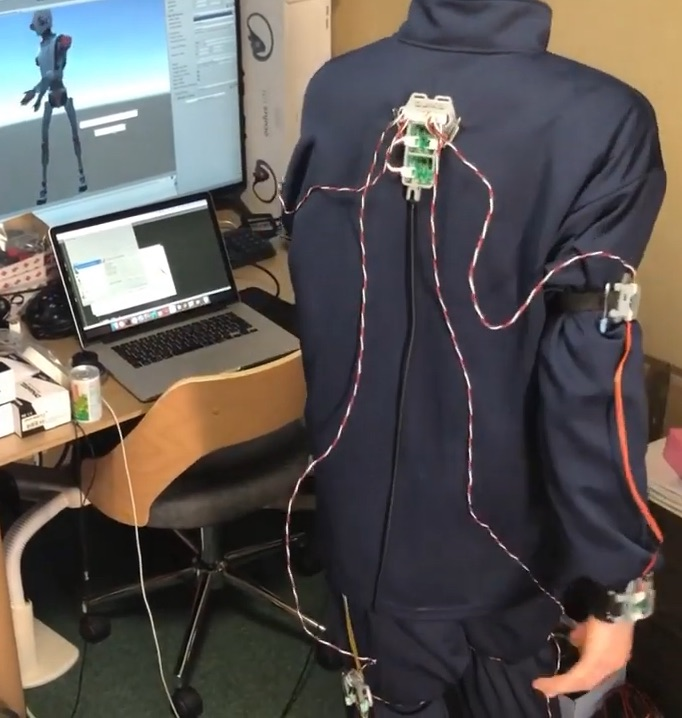
\includegraphics[width=0.45\textwidth]{testing.jpg}
    \caption{Testing scene} \label{testing}
\end{figure}
Figure \ref{testing} shows the scene of testing.
It can be seen that 3D model in the display reflects the pose of the user.
CPU usage is about \SI{20}{\percent}.

\section{Conclusion}
We propose a low-cost motion tracking system optimized for VR experience.
It only spends about 10 dollars per joint and produces 30 samples per second.
The accuracy is enough to reflect real-world movements.

Our future work is to evaluate the system quantitatively.
Developing other nodes such as wireless terminal node or position tracking node is also our future work.

\appendix
Table \ref{list} lists components of sensor node and terminal node.
The price is in USD and if you order multiple units at once, prices can be lowered.

\begin{table*}[t]
    \centering
    \caption{Component list} \label{list}
    \begin{tabular}{cccc}
        \hline
        Part & Vendor & Model & Unit Price \\ \hline
        MCU & NXP & LPC802M001JDH16FP & \$1.29 \\
        IMU & TDK & ICM-20948 & \$8.04 \\
        Regulator & Microchip & MIC5504-1.8YM5-TR & \$0.11 \\
        RS-485 Transceiver & TI & THVD1500DR & \$1.51 \\
        USB to UART Interface & FTDI & FT234XD & \$2.04 \\
        \hline
    \end{tabular}
\end{table*}

\end{document}
